\documentclass[article,12pt,onesidea,4paper,english,brazil]{abntex2}

\usepackage{lmodern, indentfirst, nomencl, color, graphicx, microtype, lipsum,textcomp}			
\usepackage[T1]{fontenc}		
\usepackage[utf8]{inputenc}		

\setlrmarginsandblock{2cm}{2cm}{*}
\setulmarginsandblock{2cm}{2cm}{*}
\checkandfixthelayout

\setlength{\parindent}{1.3cm}
\setlength{\parskip}{0.2cm}

\SingleSpacing

\begin{document}
	
	\selectlanguage{brazil}
	
	\frenchspacing 
	
	\begin{center}
		\LARGE PARÂMETROS FÍSICO-QUÍMICOS E MICROBIOLÓGICOS NO RIO MACHADO NAS IMEDIAÇÕES DA CIDADE DE JI-PARANÁ – RO\footnote{Trabalho realizado dentro da área de Conhecimento CNPq/CAPES: Ciências Exatas e da Terra com financiamento do IFRO por meio da PROPESP.}
		
		\normalsize
		Rodrigo BarrosdeOliveira\footnote{Bolsista (Ensino Superior), rodrigobrrsoliveira@gmail.com, Campus Ji-Paraná.} 
		Ingrid FerreiraChagasSoneguete\footnote{Colaborador(a), ingridferreirachagas@gmail.com , Campus Ji-Paraná.} 
		Luís Fernando LiraSouto\footnote{Orientador(a), luis.lira@ifro.edu.br, Campus Ji-Paraná.} 
		Valério MagalhãesLopes\footnote{Co-orientador(a), valerio.lopes@ifro.edu.br , Campus Ji-Paraná.} 
	\end{center}
	
	% resumo em português
	\begin{resumoumacoluna}
		A ação antrópica em rios através do lançamento de águas residuais, ocupaçãodasmargensecarreamentoderesíduosagrícolascomprometeaqualidade da água, restringindo seu uso para consumo humano. Assim a presente pesquisa objetivouavaliaralgunsparâmetrosfísico-químicosemicrobiológicosnoRioMachado em Ji-Paraná/RO. As amostras foram coletadas no período da cheia (fevereiro), vazante (abril), seca (agosto) e enchente (novembro) em 2015. Os parâmetros determinados foram pH, alcalinidade, sólidos totais e dissolvidos, turbidez, condutividade, dureza total, temperatura, coliformes totais e coliformes de origem fecal. Os resultados mostraram que as águas do rio Machado ainda não estão seriamente afetadas pelo despejo de esgoto doméstico oriundos da cidade de Ji- Paraná.
		
		\vspace{\onelineskip}
		
		\noindent
		\textbf{Palavras-chave}: Bacia amazônica. Qualidade da água. Esgoto doméstico.
		
	\end{resumoumacoluna}
	
	\section*{Introdução}
	
No Brasil são muitos os estudos relacionados à contaminação por esgotos domésticos, os quais constituem uma das principais fontes de poluição dos recursos hídricos, sendo o despejo de matéria orgânica, a principal fonte de poluiçãoantrópica por esse meio (FINOTI et al., 2009; NASCIMENTO; NAIME,2009).

Em todo o país, o tratamento de esgotos domésticos está abaixo de 25\% do total coletado, esse baixo percentual está relacionado ao custo para o tratamento de água (ANDREOLI; TORRES, 2014). Segundo o Plano Municipal de Saneamento BásicodeJi-Paraná,oprojetoderedecoletoradeesgotoprevêo
bomfuncionamento do esgotamento sanitário somente em 2041 (JI-PARANÁ,2012).

Medianteaausênciadesaneamentobásiconacidade,bemcomoalocalização doRioMachado,oqual
cruzaomunicípio,separando-oemdoisdistritos,esseestudo busca avaliar alguns parâmetros de qualidade da água nesse corpo hídrico, considerandoqueomesmorecebedesaguedecórregostributários,queao
percorrer o perímetro urbano, transportam resíduos de efluentes domésticos e industriais,além da carga orgânica in natura das comunidadesribeirinhas.

	.
	
	\section*{Material e Método}
	
	A área de estudo compreende o trecho do rio Machado que corta a cidade de Ji-Paraná, seus limites situam-se entre os paralelos 10°53'54" e 10°51'06" de latitude sul e os meridianos 61°55'18" e 61°56'30" de longitude oeste. Na Figura 1 é ilustrado o mapa amostral confeccionado com auxílio do programa livre Gvsig.
	\begin{figure}[h]
		\centering
		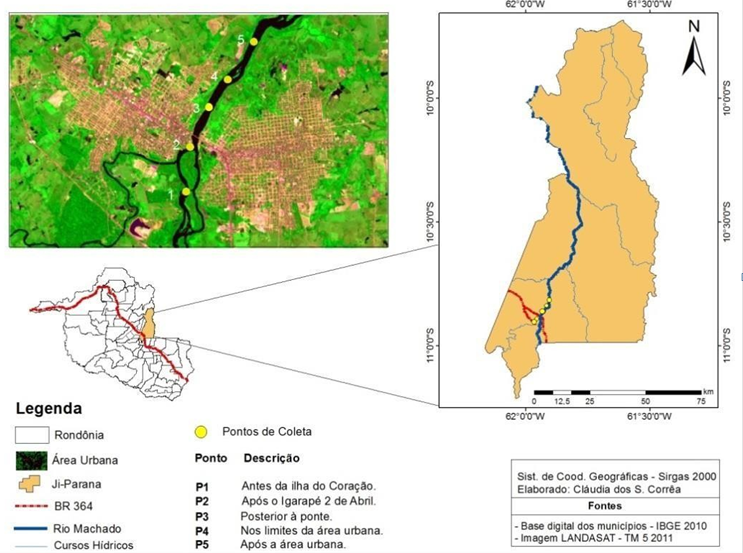
\includegraphics[width=0.7\linewidth]{pip-137-01}
		\caption{Mapa de localização dos pontos de coleta.}
	\end{figure}

Na tabela 2 encontra-se uma breve descrição de cada um dos pontos com suas respectivas coordenadas.

\begin{table}[h]
	\centering
	\caption{Descrição e localização dos pontos amostrais, onde S = Sul e O = Oeste}
	\label{my-label}
	\begin{tabular}{|l|l|l|}
		\hline
		\textbf{PONTO} & \textbf{DESCRIÇÃO}          & \textbf{COORDENADAS}     \\ \hline
		\textbf{P1}    & Antes da ilha do Coração.   & 10°53'55" S; 61°56'37" O \\ \hline
		\textbf{P2}    & Após o Igarapé 2 de Abril.  & 10°53'06" S; 61°56'29" O \\ \hline
		\textbf{P3}    & Posterior à ponte.          & 10°52'25" S; 61°56'13" O \\ \hline
		\textbf{P4}    & Nos limites da área urbana. & 10°51'50" S; 61°55'48" O \\ \hline
		\textbf{P5}    & Após a área urbana.         & 10°51'06" S; 61°55'18" O \\ \hline
	\end{tabular}
\end{table}
As campanhas de coleta foram realizadas respeitando o regime hidrológico do rio Machado, portanto, as mesmas foram efetivadas em 2015 nos meses defevereiro (período de cheia), abril (na vazante), agosto (na seca) e novembro (na época de enchente ou subida das águas). Foi realizado uma coleta a cada período em cinco pontos do rio machado, sendo a distância entre os mesmos de aproximadamente 1,5 km para abranger a cidade de Ji-Paraná às margens dorio.

Quanto às análises, as mesmas foram realizadas no Laboratório de Química Inorgânicadocâm-
pusIFROJi-Paraná,ondesedeterminouosseguintesparâmetros: pH, temperatura alcalinidade, dureza total, sólidos totais dissolvidos e sedimentáveis, condutividade, coliformes totais e coliformes termotolerantes.

Na determinação dos parâmetros, o pH foi medido por potenciometria, utilizando-seopHmetro
damarcaTepron,modeloTpH-2000.Acondutividadeelétrica foi medida por condutimetria, utilizando-se o condutivímetro da marca MS Tecnopon, modelo mCA150.

A alcalinidade foi medida por titulação potenciométrica, tendo sindo utilizadas as seguintes soluções: solução de ácido sulfúrico 0,02 N e a solução indicadora de verde de bromocresol/vermelho de metila. Para a análise da turbidez foi utilizado o turbidímetro da marca HANNA, modelo HI 93703, devidamente calibrado. Cada amostra foi colocada dentro dos cilindros de vidro até a marca indicada no mesmo e foi introduzida no turbidímetro para a realização da leitura.

A dureza da água foi medida por titulação potenciométrica, sendo usado como solução o EDTA 0,01 M, uma solução tampão e o indicador eriochrome black T. Os sólidos sedimentáveis foram determinados por meio de gravimetria, usando conesde Imhoff.


Para a análise microbiológica foi utilizado frascos de vidro scott autoclavados por15minutosà
umatemperaturade121ºC,empregandoatécnicadetubosmúltiplos conforme a metodologia descrita em APHA et al. (2005), onde foi utilizado os seguintesmeiosdecultura:LactoseBroth(HIMEDIA),paraotes-
tepresuntivo;Brilliant Green Bile Broth (ACUMEDIA), para identificação de coliformes totais e EC Broth (HIMEDIA), para a identificação de coliformes termotolerantes. Os resultados foram dados em Número Mais Provável (NMP), conforme manual da CETESB(2015).

	
	\section*{Resultados e Discussão}
	
	
A portaria n° 518/2004 do Ministério da Saúde, estabelece como padrão de potabilidadedaáguaparaconsumohumanoafaixadepHentre6,0a9,5,econforme aresoluçãon°357/2005doCONAMA,para
riosdeáguadoceclasse2,afaixadepH deve estar entre 6,0 a 9,0 (Figura 2). Durante todos os regimes hidrológicos, o pH manteve-se próximo à neutralidade, na cheia e enchente respectivamente foram medidososvaloresmaiselevadosparaesseparâmetro.Carvalhoetal(2000)explica queoaumentodopHduranteaenchenteestárelacionadoháumamaiordiluiçãodos compostos dissolvidos, o que provoca a redução daacidez.

	\begin{figure}[!h]
	\centering
	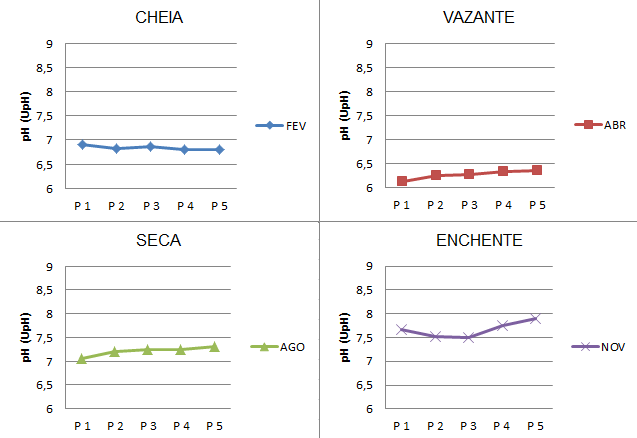
\includegraphics[width=.8\linewidth]{pip-137-02}
	\caption{pH durante os regimes hidrológicos.}
\end{figure}

A alcalinidade manteve-se entre 10,09 a 15,96 mg de CaCO3/L, sendo que os maiores valores ocorreram na seca (Figura 3), acompanhando o pH alcalino, comportamento similar ao encontrado por Furtado (2005) no rio Acre, em Rio Branco, que ocorre devido à baixa pluviosidade característica do período da seca, favorecendo a concentração de íons presentes nos efluentes. A resolução do CONAMA n° 357/2005 não estabelece um padrão para o teor de alcalinidade para a classificação do rio em classe.

	\begin{figure}[!h]
	\centering
	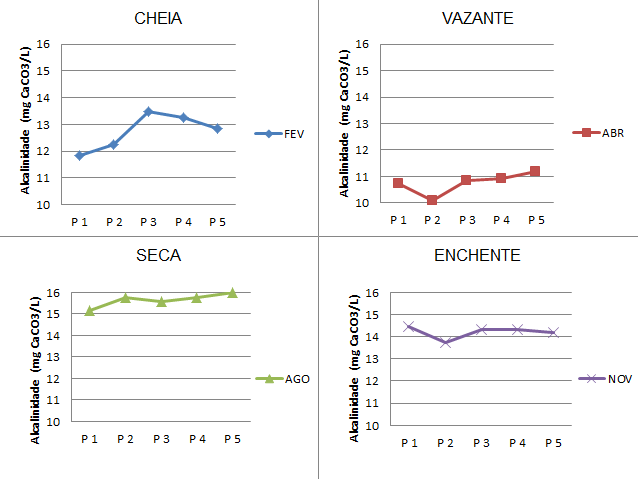
\includegraphics[width=0.8\linewidth]{pip-137-03}
	\caption{Alcalinidade durante os regimes hidrológicos.}
	\end{figure}

Águas que apresentam valores abaixo de 50 mg/L CaCO3 são consideradas mole e tem grande proveito para a utilização direta, já para valores acima de 150 mg/L CaCO3 é considerada dura e requer tratamento de abrandamento para determinadas finalidades (LIBÂNIO, 2005). Os resultados obtidos para a dureza total ficaram abaixo do limite máximo permitido (Figura 4) se comparado com a portaria nº 518/2004 do Ministério da Saúde que estabelece 500 mg/L CaCO3 para águas de consumo humano.

\begin{figure}[!h]
	\centering
	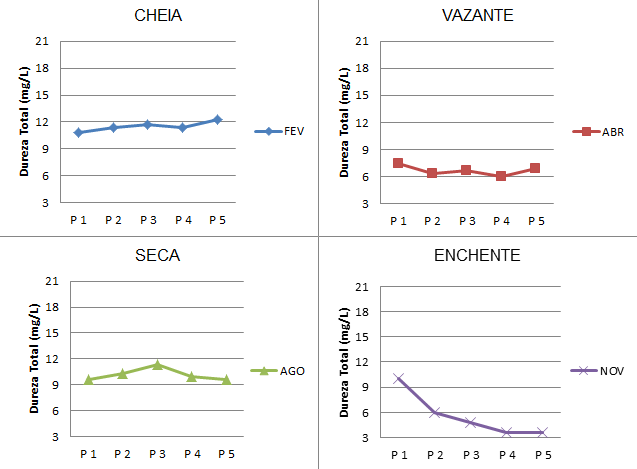
\includegraphics[width=0.8\linewidth]{pip-137-04}
	\caption{Dureza Total durante os regimes hidrológicos.}
\end{figure}

Em todos os pontos, a condutividade esteve abaixo de 100 $\mu$ S cm-¹ (Figura 5), atendendo a resolução do Ministério da Saúde (BRASIL, 2006). Em estudos no Rio Jamari, em Rondônia, Lemos (2007) também encontra valores menores de condutividade durante a seca e maiores durante a enchente.

\begin{figure}[!h]
	\centering
	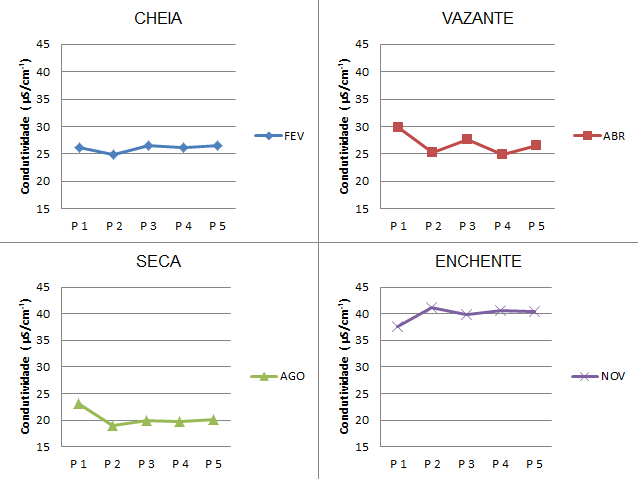
\includegraphics[width=0.8\linewidth]{pip-137-05}
	\caption{Condutividade durante os regimes hidrológicos.}
\end{figure}

Brigante e Espindola (2003) explica que para águas naturais, a condutividade elétrica fica na faixa de 10 a 100 $\mu$ S cm-¹ e para ambientes poluídos por esgoto doméstico ou industrial, esses valores podem chegar a 1000 $\mu$ S cm-¹.

Não houve uma variação considerável de sólidos totais dissolvidos entre os ciclos hidrológicos, permanecendo estes na faixa de 9,26 a 13,92 mg/L, sendo que o ponto 5 obteve o maior valor em todos os períodos (Figura 6). Seguindo a classificação do CONAMA 357(2005), para este quesito, o Rio Machado se enquadra na classe 1, pois apresenta valores inferiores a 500 mg/L.

\begin{figure}[!h]
	\centering
	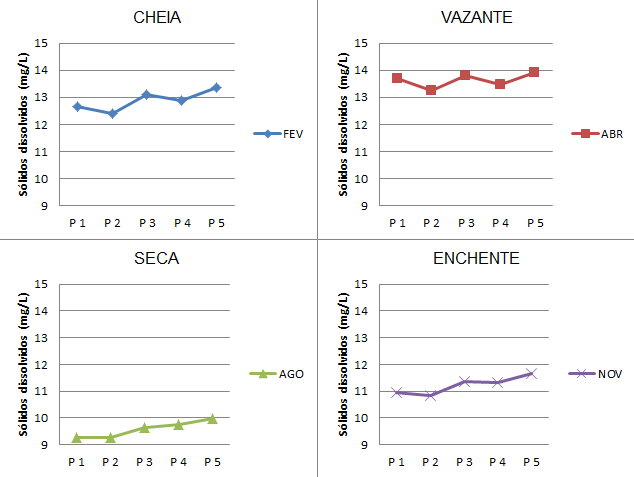
\includegraphics[width=0.8\linewidth]{pip-137-06}
	\caption{Sólidos totais dissolvidos durante os regimes hidrológicos.}
\end{figure}

De forma geral os sólidos sedimentáveis mantiveram-se na média de 0,235 mg/L, tendo um aumento significativo durante a cheia, devido ao carreamento de solos, material orgânico e outras partículas. Do ponto 4 ao ponto 5, pode se observar uma progressão nos valores na maioria dos períodos (Figura 7), tal fato pode estar relacionado às atividades de extração de areia desenvolvidas nesta área.

\begin{figure}[!h]
	\centering
	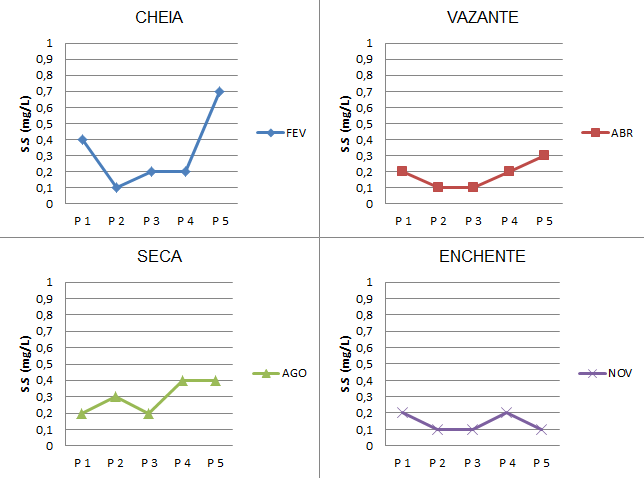
\includegraphics[width=0.8\linewidth]{pip-137-07}
	\caption{Sólidos sedimentáveis durante os regimes hidrológicos.}
\end{figure}

A temperatura teve uma variação média de 2,4 °C, observando um aumento da temperatura entre os períodos de seca e enchente, caracterizados pela alta intensidade dos raios solares. Souto (2014) verificou o mesmo comportamento térmico em seu estudo no Rio Solimões, no Amazonas. Conforme Esteves (1998), rios de regiões tropicais apresentam temperaturas altas e constantes, e ocorre pouca variação térmica entre os períodos.

Quanto à turbidez, no período da cheia houve um aumento considerável em relação ao período da seca (Figura 8), o que era esperado, visto que na cheia ocorre o carreamento de material sólido para o leito do rio e na seca há a sedimentação de sólidos associado à baixa vazão. Num estudo sobre as bacias hidrográficas de Rondônia, Zuffo et al. (2013) encontraram os valores mais baixos de turbidez para a bacia hidrográfica do Rio Machado nas duas campanhas de coleta. A resolução n° 357/2005 do CONAMA, limita a turbidez de corpos d´água para classe 1 com no máximo 40 UNT e para classe 2 até 100 UNT. Apesar de possuir uma grande variação nos valores durante os ciclos hidrológicos, o Rio Machado manteve-se abaixo dos 40 UNT na média geral.

\begin{figure}[!h]
	\centering
	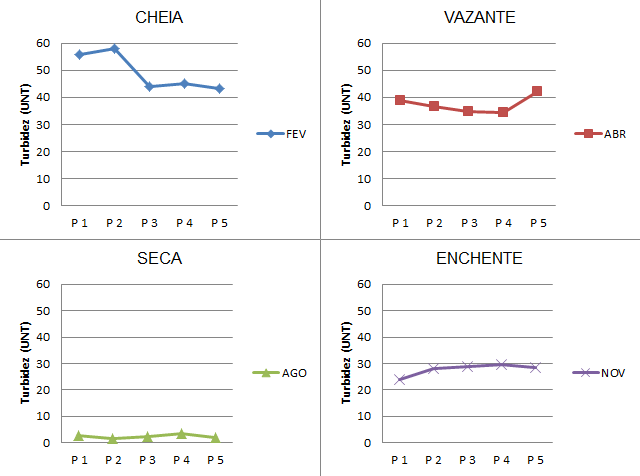
\includegraphics[width=0.8\linewidth]{pip-137-08}
	\caption{Turbidez durante os regimes hidrológicos.}
\end{figure}

Coliformes totais estão associados a um grupo mais amplo de bactérias presentes também no solo e na vegetação (LIBÂNIO, 2005; MACÊDO, 2007). No período das águas altas (enchente/cheia), foi encontrado os maiores valores (Figura 9).

\begin{figure}[!h]
	\centering
	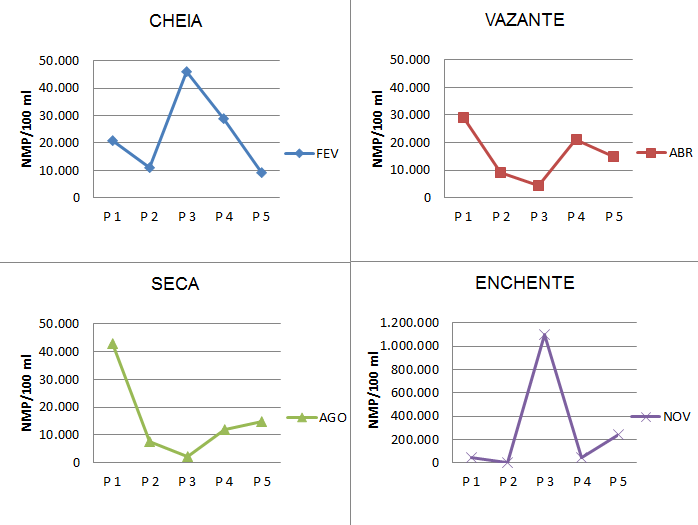
\includegraphics[width=0.8\linewidth]{pip-137-09}
	\caption{Coliformes totais durante os regimes hidrológico.}
\end{figure}

No ponto 3 obteve-se a maior média para coliformes totais, o que pode ter relação com a área assoreada onde ele se localiza, pela influência antrópica e também por estar a jusante do Igarapé Dois de Abril.

Quanto aos coliformes termotolerantes, durante o período da seca pode se observar baixos valores, na faixa de 36 a 430 NMP/100 ml, com uma média de 200 NMP/100 ml (Figura 10), o que pode ser justificado pela ausência de precipitação neste período, evitando carreamento de dejetos e matéria orgânica para o leito do rio, além de contribuir para a decantação de sólidos.

\begin{figure}[!h]
	\centering
	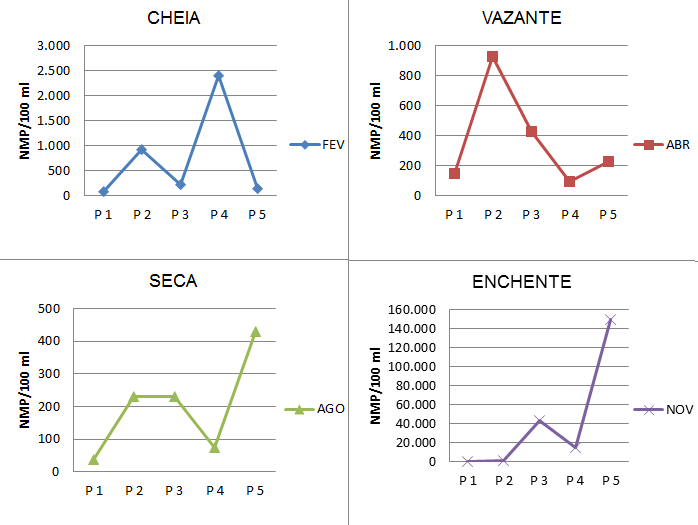
\includegraphics[width=0.8\linewidth]{pip-137-10}
	\caption{Coliformes termotolerantes durante os regimes hidrológicos.}
\end{figure}

Segundo a resolução n° 357/2005 (CONAMA, 2005) para os demais usos além de recreação de contato secundário e para dessedentação de animais criados confinados, o limite máximo permitido de coliformes termotolerantes para águas doces classe I, II e III é de 200, 1000 e 4000 NMP respectivamente por 100 mililitros em 80\% ou mais, de pelo menos 6 amostras, coletadas durante o período de um ano, com frequência bimestral. Apenas os pontos 1 e 2 ficaram com médias abaixo de 1000 NMP/100 ml nas análises durante os ciclos hidrológicos, enquanto os pontos 3, 4 e 5 atingiram médias acima dos limites estabelecidos pela legislação. Esse fato pode estar associado à incidência de chuvas no período da enchente, ocasionando o carreamento de dejetos no leito do rio, visto que nos demais períodos, a média foi satisfatória.

	\section*{Conclusões}
	
	O rio Machado apresentou comportamento distinto nos ciclos hidrológicos, mostrando uma variabilidade nos parâmetros analisados, principalmente na turbidez, condutividade elétrica, coliformes totais e nos coliformes de origem fecal. Todos os parâmetros físico-químicos analisados durante os períodos permaneceram dentro dos padrões estipulados pelas normas vigentes, indicando a ausência de grandes atividades industriais, geradoras de resíduos sólidos. Quanto às análises microbiológicas, os valores que ficaram fora dos parâmetros, ocorreram na subida das águas (cheia e enchente) devido ao carreamento de materiais sólidos e dejetos ao leito do rio. Destaca-se também a capacidade de autodepuração do rio Machado, dado que a cidade de Ji-Paraná ainda não possui rede de tratamento de esgoto, ocasionando o lançamento de efluentes domésticos em córregos, que por sua vez chega ao rio, deste modo, os resultados mostraram que o rio ainda não está seriamente afetado pelo despejo de efluentes doméstico in natura, contudo falta políticas públicas que promovam a conservação dos recursos hídricos bem como a biodiversidade local, visto que a cidade de Ji-Paraná é cortada pelo rio Machado e recebe diretamente influencia antrópica.
	
	\section*{Agradecimentos}
	
	Ao IFRO/PROPESP e ao CNPq pelo apoio institucional e financeiro.
	
	\section*{Instituição de Fomento}
	
	IFRO e CNPq.
	
	\section*{Referências}
	
ANDREOLI, C. V.; TORRES, P. L. A relação da qualidade e quantidade da água no ambiente urbano e rural. In: Complexidade: redes e conexões do ser sustentável. Curitiba : SENAR, 2014. 832 p.

APHA; AWWA; WEF. Multiple tube fermentation technique for members of the coliform group. In: . \textbf{Standard Methods for the Examination of Water and Wastewater}. 21st ed. Washington DC: APHA, 2005. Section 9221.

JI-PARANÁ. Plano municipal de saneamento básico de Ji-Paraná/RO. 2012.
Disponível em: < http://www.ji-parana.ro.gov.br/pub-leis/saneamento/RELATORIO
\_REV014-1[1].pdf >. Acesso em: 04 fev. 2016.

BRASIL. Lei n. 12.651, de 25 de março de 2012. Dispõe sobre a proteção da vegetação nativa. Disponível em: <http://www.planalto.gov.br/ccivil\_03/\_ato2011- 2014/2012/lei/l12651.htm>. Acesso em: 17 mar. 2016.

BRIGANTE, J.; ESPINDOLA, E. L. G. Limnologia fluvial – um estudo no Rio Mogi- Guaçu. São Carlos: Rima, 2003. 255p.

CARVALHO, A. R.; SCHLITTLER, F. H. M.; TORNISIELO, V. L. Relações da
atividade agropecuária com parâmetros físicos químicos da água. Química Nova. v.23, n. 5, p. 618-622, 2000.

CETESB. Companhia de Tecnologia de Saneamento Ambiental de São Paulo. Disponível em: <http://www.cetesb.sp.gov.br/userfiles/file/agua/aguas- superficiais/aguas-interiores/variaveis/aguas/variaveis\_microbiologicas/ coliformes\_termotolerantes.pdf >. Acesso em 17 mar. 2015.

ESTEVES, F. A. Fundamentos de Limnologia. 2. ed., Rio de Janeiro: Interciência, 1998. 602p.

FURTADO, C. M. Caracterização limnológica e avaliação da qualidade da água de um trecho urbano do Rio Acre, Rio Branco-Ac, Brasil. 2005. 58f. Dissertação (Mestrado em Ecologia e Manejo de Recursos Naturais) - Universidade Federal do Acre, Rio Branco, 2005.

LEMOS, R. N. S. Monitoramento da Ictiofauna do Rio Jamari a montante e jusante da UHE de Samuel-RO. 2007. 203f. Dissertação (Mestrado em Desenvolvimento Regional e Meio Ambiente) - Universidade Federal de Rondônia, 2007.

LIBÂNIO, M. Fundamentos de qualidade e tratamento de água. Campinas: Átomo, 2005.
MACÊDO, J. A. B. Águas e Águas – Doenças de veiculação hídrica e alimentar. 3.ed. Belo Horizonte: CRQ-MG, 2007. Disponível em: <www.jorgemacedo.pro.br>. Acessado em: 12 fev. 2016.

MOURA, A. C.; ASSUMPÇÃO R. A. B.; BISCHOFF, J. Monitoramento físico-químico e microbiológico da água do Rio Cascavel durante o período de 2003 a 2006. Arq.
Inst. Biol, São Paulo, v.76, n.1, p.17-22, 2009.

NASCIMENTO, C.A.; NAIME, R. Panorama do uso, distribuição e contaminação das águas superficiais no Arroio Pampa na bacia do Rio dos Sinos. Estudos Tecnológicos, v. 5, n. 1, p. 101-120, 2009.

SOUTO, L. F. L. Análise espaço-temporal de elementos maiores e variáveis físico-químicas em um trecho do Rio Solimões-Amazonas. 2014. 80f.
Dissertação (Mestrado em Química) - Instituto de Ciências Exatas, Universidade Federal do Amazonas. 2014.

ZUFFO, C. E. et al. Caracterização da Qualidade de Águas Superficiais em Rondônia. Anuário do Instituto de Geociências, v. 36, n. 2, p. 25-39, 2013.
	
\end{document}
